\begin{enumerate}[label=\thesection.\arabic*.,ref=\thesection.\theenumi]
\numberwithin{equation}{enumi}

\textit{Question:} Consider the following asymptotic Bode magnitude plot ($\omega$ is in rad/s).
\begin{center}
      \begin{figure}[!h]
      \centering
      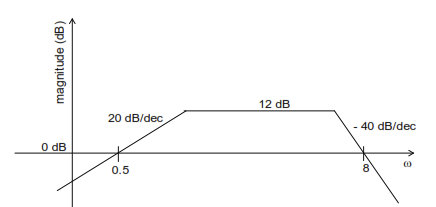
\includegraphics[width=\columnwidth]{./figs/ep18btech11016_fig1.png}
      \caption{Plot of G(s)}
      \label{fig:ep18btech11016_fig1}
      \end{figure}
\end{center}

Which of the following transfer function is best represented by the above Bode magnitude plot?
\begin{multline*}
    (A) \cfrac{2s}{(1+0.5s)(1+0.25s)^2}\hspace{0.5cm}
    (B) \cfrac{4(1+0.5s)}{s(1+0.25s)}
\end{multline*}
\begin{multline*}
    (C) \cfrac{2s}{(1+2s)(1+4s)}\hspace{0.5cm}
    (D) \cfrac{4s}{(1+2s)(1+4s)^2}
\end{multline*}

By looking to the plot, we can say that since the initial slope is +20, there must be a zero at the origin.
Let the corner frequencies of the plot be $\omega_{01}$ and $\omega_{02}$. They can be calculated as follows:
\begin{align*}
    slope = \cfrac{M_2 - M_1}{log\omega_2 - log\omega_1}\\
\end{align*}
Therefore for $\omega_{02}$,\\
-40 = \cfrac{0 - 12}{log8 - log\omega_{02}}\\
log8 - log$\omega$_{02} = \cfrac{12}{40}\\
log$\omega_{02}$ = log8 - \cfrac{12}{40}\\
$\omega_{02}$ = 4\\

And for $\omega_{01}$,\\
20 = \cfrac{0 - 12}{log0.5 - log$\omega_{01}$}\\
log0.5 - log$\omega_{01}$ = \cfrac{-12}{20}\\
log$\omega_{01}$ = log0.5 + \cfrac{12}{20}\\
$\omega_{01}$ = 2\\
So, the corner frequencies are $\omega_{01}$=2 and $\omega_{02}$ = 4.
At $\omega_{01}$, the change in slope is -20dB, so their exists one pole at this frequency and at $\omega_{02}$, the change in slope is -40dB, so their exists two pole at this frequency.\\
The denominators have the form (1 + \cfrac{s}{\omega})

So, the denominator of the transfer function is\\ $(1 + \cfrac{s}{2})(1 + \cfrac{s}{4})^2$\\
Therefore, the transfer function is,
\begin{align*}
    \cfrac{cs}{(1 + \cfrac{s}{2})(1 + \cfrac{s}{4})^2} 
\end{align*}
here c is some constant\\
The answer is therefore option (A)
\begin{align*}
     \cfrac{2s}{(1+0.5s)(1+0.25s)^2}
\end{align*}{}

We will now plot the bode plot of the given transfer function to verify it.
The bode plot is:
\begin{center}
    \begin{figure}[!h]
    \centering
    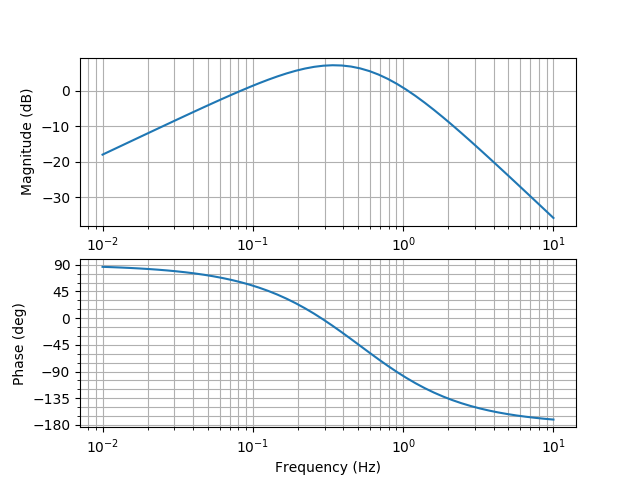
\includegraphics[width=\columnwidth]{./figs/ep18btech11016_fig2.png}
    \caption{Plot of G(s)}
    \label{fig:ep18btech11016_fig2}
    \end{figure}
\end{center}
The plot was plotted using the following code:
\lstinputlisting{./codes/ep18btech11016.py}

\end{enumerate}
